% Options for packages loaded elsewhere
\PassOptionsToPackage{unicode}{hyperref}
\PassOptionsToPackage{hyphens}{url}
\PassOptionsToPackage{dvipsnames,svgnames,x11names}{xcolor}
%
\documentclass[
  a4paper,
]{article}

\usepackage{amsmath,amssymb}
\usepackage{iftex}
\ifPDFTeX
  \usepackage[T1]{fontenc}
  \usepackage[utf8]{inputenc}
  \usepackage{textcomp} % provide euro and other symbols
\else % if luatex or xetex
  \usepackage{unicode-math}
  \defaultfontfeatures{Scale=MatchLowercase}
  \defaultfontfeatures[\rmfamily]{Ligatures=TeX,Scale=1}
\fi
\usepackage{lmodern}
\ifPDFTeX\else  
    % xetex/luatex font selection
\fi
% Use upquote if available, for straight quotes in verbatim environments
\IfFileExists{upquote.sty}{\usepackage{upquote}}{}
\IfFileExists{microtype.sty}{% use microtype if available
  \usepackage[]{microtype}
  \UseMicrotypeSet[protrusion]{basicmath} % disable protrusion for tt fonts
}{}
\makeatletter
\@ifundefined{KOMAClassName}{% if non-KOMA class
  \IfFileExists{parskip.sty}{%
    \usepackage{parskip}
  }{% else
    \setlength{\parindent}{0pt}
    \setlength{\parskip}{6pt plus 2pt minus 1pt}}
}{% if KOMA class
  \KOMAoptions{parskip=half}}
\makeatother
\usepackage{xcolor}
\usepackage[top=2.54cm,right=2.54cm,bottom=2.54cm,left=2.54cm]{geometry}
\setlength{\emergencystretch}{3em} % prevent overfull lines
\setcounter{secnumdepth}{-\maxdimen} % remove section numbering
% Make \paragraph and \subparagraph free-standing
\ifx\paragraph\undefined\else
  \let\oldparagraph\paragraph
  \renewcommand{\paragraph}[1]{\oldparagraph{#1}\mbox{}}
\fi
\ifx\subparagraph\undefined\else
  \let\oldsubparagraph\subparagraph
  \renewcommand{\subparagraph}[1]{\oldsubparagraph{#1}\mbox{}}
\fi

\usepackage{color}
\usepackage{fancyvrb}
\newcommand{\VerbBar}{|}
\newcommand{\VERB}{\Verb[commandchars=\\\{\}]}
\DefineVerbatimEnvironment{Highlighting}{Verbatim}{commandchars=\\\{\}}
% Add ',fontsize=\small' for more characters per line
\newenvironment{Shaded}{}{}
\newcommand{\AlertTok}[1]{\textcolor[rgb]{1.00,0.33,0.33}{\textbf{#1}}}
\newcommand{\AnnotationTok}[1]{\textcolor[rgb]{0.42,0.45,0.49}{#1}}
\newcommand{\AttributeTok}[1]{\textcolor[rgb]{0.84,0.23,0.29}{#1}}
\newcommand{\BaseNTok}[1]{\textcolor[rgb]{0.00,0.36,0.77}{#1}}
\newcommand{\BuiltInTok}[1]{\textcolor[rgb]{0.84,0.23,0.29}{#1}}
\newcommand{\CharTok}[1]{\textcolor[rgb]{0.01,0.18,0.38}{#1}}
\newcommand{\CommentTok}[1]{\textcolor[rgb]{0.42,0.45,0.49}{#1}}
\newcommand{\CommentVarTok}[1]{\textcolor[rgb]{0.42,0.45,0.49}{#1}}
\newcommand{\ConstantTok}[1]{\textcolor[rgb]{0.00,0.36,0.77}{#1}}
\newcommand{\ControlFlowTok}[1]{\textcolor[rgb]{0.84,0.23,0.29}{#1}}
\newcommand{\DataTypeTok}[1]{\textcolor[rgb]{0.84,0.23,0.29}{#1}}
\newcommand{\DecValTok}[1]{\textcolor[rgb]{0.00,0.36,0.77}{#1}}
\newcommand{\DocumentationTok}[1]{\textcolor[rgb]{0.42,0.45,0.49}{#1}}
\newcommand{\ErrorTok}[1]{\textcolor[rgb]{1.00,0.33,0.33}{\underline{#1}}}
\newcommand{\ExtensionTok}[1]{\textcolor[rgb]{0.84,0.23,0.29}{\textbf{#1}}}
\newcommand{\FloatTok}[1]{\textcolor[rgb]{0.00,0.36,0.77}{#1}}
\newcommand{\FunctionTok}[1]{\textcolor[rgb]{0.44,0.26,0.76}{#1}}
\newcommand{\ImportTok}[1]{\textcolor[rgb]{0.01,0.18,0.38}{#1}}
\newcommand{\InformationTok}[1]{\textcolor[rgb]{0.42,0.45,0.49}{#1}}
\newcommand{\KeywordTok}[1]{\textcolor[rgb]{0.84,0.23,0.29}{#1}}
\newcommand{\NormalTok}[1]{\textcolor[rgb]{0.14,0.16,0.18}{#1}}
\newcommand{\OperatorTok}[1]{\textcolor[rgb]{0.14,0.16,0.18}{#1}}
\newcommand{\OtherTok}[1]{\textcolor[rgb]{0.44,0.26,0.76}{#1}}
\newcommand{\PreprocessorTok}[1]{\textcolor[rgb]{0.84,0.23,0.29}{#1}}
\newcommand{\RegionMarkerTok}[1]{\textcolor[rgb]{0.42,0.45,0.49}{#1}}
\newcommand{\SpecialCharTok}[1]{\textcolor[rgb]{0.00,0.36,0.77}{#1}}
\newcommand{\SpecialStringTok}[1]{\textcolor[rgb]{0.01,0.18,0.38}{#1}}
\newcommand{\StringTok}[1]{\textcolor[rgb]{0.01,0.18,0.38}{#1}}
\newcommand{\VariableTok}[1]{\textcolor[rgb]{0.89,0.38,0.04}{#1}}
\newcommand{\VerbatimStringTok}[1]{\textcolor[rgb]{0.01,0.18,0.38}{#1}}
\newcommand{\WarningTok}[1]{\textcolor[rgb]{1.00,0.33,0.33}{#1}}

\providecommand{\tightlist}{%
  \setlength{\itemsep}{0pt}\setlength{\parskip}{0pt}}\usepackage{longtable,booktabs,array}
\usepackage{calc} % for calculating minipage widths
% Correct order of tables after \paragraph or \subparagraph
\usepackage{etoolbox}
\makeatletter
\patchcmd\longtable{\par}{\if@noskipsec\mbox{}\fi\par}{}{}
\makeatother
% Allow footnotes in longtable head/foot
\IfFileExists{footnotehyper.sty}{\usepackage{footnotehyper}}{\usepackage{footnote}}
\makesavenoteenv{longtable}
\usepackage{graphicx}
\makeatletter
\def\maxwidth{\ifdim\Gin@nat@width>\linewidth\linewidth\else\Gin@nat@width\fi}
\def\maxheight{\ifdim\Gin@nat@height>\textheight\textheight\else\Gin@nat@height\fi}
\makeatother
% Scale images if necessary, so that they will not overflow the page
% margins by default, and it is still possible to overwrite the defaults
% using explicit options in \includegraphics[width, height, ...]{}
\setkeys{Gin}{width=\maxwidth,height=\maxheight,keepaspectratio}
% Set default figure placement to htbp
\makeatletter
\def\fps@figure{htbp}
\makeatother

\makeatletter
\makeatother
\makeatletter
\makeatother
\makeatletter
\@ifpackageloaded{caption}{}{\usepackage{caption}}
\AtBeginDocument{%
\ifdefined\contentsname
  \renewcommand*\contentsname{Tabla de contenidos}
\else
  \newcommand\contentsname{Tabla de contenidos}
\fi
\ifdefined\listfigurename
  \renewcommand*\listfigurename{Listado de Figuras}
\else
  \newcommand\listfigurename{Listado de Figuras}
\fi
\ifdefined\listtablename
  \renewcommand*\listtablename{Listado de Tablas}
\else
  \newcommand\listtablename{Listado de Tablas}
\fi
\ifdefined\figurename
  \renewcommand*\figurename{Figura}
\else
  \newcommand\figurename{Figura}
\fi
\ifdefined\tablename
  \renewcommand*\tablename{Tabla}
\else
  \newcommand\tablename{Tabla}
\fi
}
\@ifpackageloaded{float}{}{\usepackage{float}}
\floatstyle{ruled}
\@ifundefined{c@chapter}{\newfloat{codelisting}{h}{lop}}{\newfloat{codelisting}{h}{lop}[chapter]}
\floatname{codelisting}{Listado}
\newcommand*\listoflistings{\listof{codelisting}{Listado de Listados}}
\makeatother
\makeatletter
\@ifpackageloaded{caption}{}{\usepackage{caption}}
\@ifpackageloaded{subcaption}{}{\usepackage{subcaption}}
\makeatother
\makeatletter
\@ifpackageloaded{tcolorbox}{}{\usepackage[skins,breakable]{tcolorbox}}
\makeatother
\makeatletter
\@ifundefined{shadecolor}{\definecolor{shadecolor}{rgb}{.97, .97, .97}}
\makeatother
\makeatletter
\makeatother
\makeatletter
\makeatother
\ifLuaTeX
\usepackage[bidi=basic]{babel}
\else
\usepackage[bidi=default]{babel}
\fi
\babelprovide[main,import]{spanish}
% get rid of language-specific shorthands (see #6817):
\let\LanguageShortHands\languageshorthands
\def\languageshorthands#1{}
\ifLuaTeX
  \usepackage{selnolig}  % disable illegal ligatures
\fi
\usepackage[]{biblatex}
\addbibresource{../../../../references.bib}
\IfFileExists{bookmark.sty}{\usepackage{bookmark}}{\usepackage{hyperref}}
\IfFileExists{xurl.sty}{\usepackage{xurl}}{} % add URL line breaks if available
\urlstyle{same} % disable monospaced font for URLs
\hypersetup{
  pdftitle={Introducción a la visualización de datos con python},
  pdfauthor={Edison Achalma},
  pdflang={es},
  colorlinks=true,
  linkcolor={blue},
  filecolor={Maroon},
  citecolor={Blue},
  urlcolor={Blue},
  pdfcreator={LaTeX via pandoc}}

\title{Introducción a la visualización de datos con python}
\usepackage{etoolbox}
\makeatletter
\providecommand{\subtitle}[1]{% add subtitle to \maketitle
  \apptocmd{\@title}{\par {\large #1 \par}}{}{}
}
\makeatother
\subtitle{Explora los conceptos básicos y las bibliotecas populares para
crear gráficos impactantes y comprensibles.}
\author{Edison Achalma}
\date{2023-06-29}

\begin{document}
\maketitle
\ifdefined\Shaded\renewenvironment{Shaded}{\begin{tcolorbox}[frame hidden, interior hidden, breakable, borderline west={3pt}{0pt}{shadecolor}, sharp corners, enhanced, boxrule=0pt]}{\end{tcolorbox}}\fi

\hypertarget{introducciuxf3n-a-los-gruxe1ficos-con-python}{%
\section{Introducción a los gráficos con
Python}\label{introducciuxf3n-a-los-gruxe1ficos-con-python}}

\hypertarget{por-quuxe9-los-gruxe1ficos-son-importantes-en-el-anuxe1lisis-de-datos}{%
\subsection{¿Por qué los gráficos son importantes en el análisis de
datos?}\label{por-quuxe9-los-gruxe1ficos-son-importantes-en-el-anuxe1lisis-de-datos}}

Cuando nos enfrentamos a un conjunto de datos, a veces puede resultar
abrumador tratar de extraer información significativa y comprender
patrones importantes. Aquí es donde entran en juego los gráficos. Los
gráficos son una herramienta visual poderosa que nos permite representar
datos de manera clara y comprensible.

Imagina esto: en lugar de mirar una larga lista de números o leer tablas
extensas, puedes ver tus datos plasmados en un gráfico colorido y fácil
de interpretar. Los gráficos nos permiten visualizar tendencias,
comparar valores y descubrir relaciones ocultas entre variables. Son
como una ventana que nos permite explorar y comprender los datos de
manera más intuitiva.

Los gráficos no solo hacen que el análisis de datos sea más accesible,
sino que también nos ayudan a comunicar nuestros hallazgos de manera
efectiva. Una imagen vale más que mil palabras, ¿verdad? Al presentar
información a través de gráficos, podemos transmitir mensajes complejos
de manera clara y concisa, lo que facilita que otras personas comprendan
nuestros resultados.

\hypertarget{ventajas-de-utilizar-python-para-crear-gruxe1ficos}{%
\subsection{Ventajas de utilizar Python para crear
gráficos}\label{ventajas-de-utilizar-python-para-crear-gruxe1ficos}}

Cuando se trata de crear gráficos, Python ofrece una serie de ventajas
que lo convierten en una herramienta popular y poderosa en el análisis
de datos. Veamos algunas de estas ventajas:

\begin{enumerate}
\def\labelenumi{\arabic{enumi}.}
\item
  \textbf{Facilidad de uso}: Python es un lenguaje de programación de
  alto nivel y fácil de aprender. Su sintaxis clara y legible permite a
  los usuarios escribir código de forma concisa y comprensible. Esto
  facilita la creación de gráficos, incluso para aquellos que no tienen
  experiencia previa en programación.
\item
  \textbf{Gran cantidad de bibliotecas}: Python cuenta con una amplia
  gama de bibliotecas especializadas en la visualización de datos.
  Algunas de las más populares son Matplotlib, Seaborn y Plotly. Estas
  bibliotecas ofrecen una variedad de estilos de gráficos, opciones de
  personalización y herramientas interactivas para explorar y presentar
  tus datos de manera efectiva.
\item
  \textbf{Compatibilidad con otras herramientas}: Python se integra
  fácilmente con otras herramientas y bibliotecas utilizadas en el
  análisis de datos. Puedes combinar el poder de Python con bibliotecas
  como Pandas para el procesamiento de datos, NumPy para operaciones
  numéricas y SciPy para análisis científico. Esta interoperabilidad
  facilita la manipulación y preparación de datos antes de crear tus
  gráficos.
\item
  \textbf{Comunidad activa}: Python cuenta con una gran comunidad de
  desarrolladores y usuarios que constantemente contribuyen con nuevas
  funcionalidades, mejoras y ejemplos de uso. Esto significa que siempre
  encontrarás recursos, tutoriales y soporte disponibles para ayudarte a
  resolver cualquier problema o desafío que encuentres al crear tus
  gráficos.
\item
  \textbf{Flexibilidad y versatilidad}: Python te permite crear una
  amplia variedad de gráficos, desde simples diagramas de barras hasta
  complejas visualizaciones en 3D. Puedes adaptar tus gráficos a tus
  necesidades específicas y personalizarlos con colores, etiquetas,
  leyendas y más. Además, puedes exportar tus gráficos en varios
  formatos de imagen o incrustarlos en informes y aplicaciones.
\end{enumerate}

\hypertarget{bibliotecas-populares-para-gruxe1ficos-en-python}{%
\section{Bibliotecas populares para gráficos en
Python}\label{bibliotecas-populares-para-gruxe1ficos-en-python}}

Afortunadamente, Python cuenta con varias bibliotecas populares que
facilitan la creación de gráficos de calidad. Aquí te presentamos
algunas de las más utilizadas:

\hypertarget{matplotlib}{%
\subsection{Matplotlib}\label{matplotlib}}

Matplotlib es una biblioteca ampliamente utilizada y flexible que
proporciona una gran variedad de funciones y estilos para crear gráficos
estáticos. Es una excelente opción para aquellos que desean un control
detallado sobre la apariencia de sus visualizaciones.

\hypertarget{seaborn}{%
\subsection{Seaborn}\label{seaborn}}

Seaborn es una biblioteca basada en Matplotlib que simplifica la
creación de gráficos estéticamente agradables. Ofrece una interfaz de
alto nivel y opciones predefinidas para la visualización de datos
estadísticos y de análisis exploratorio.

\hypertarget{plotly}{%
\subsection{Plotly}\label{plotly}}

Plotly es una biblioteca interactiva que permite crear gráficos
interactivos y dinámicos, incluyendo gráficos en 3D, diagramas de
dispersión animados y mapas interactivos. Además, ofrece opciones de
visualización en la web y la posibilidad de compartir tus gráficos en
línea.

\hypertarget{bokeh}{%
\subsection{Bokeh}\label{bokeh}}

Bokeh es otra biblioteca de visualización interactiva que se centra en
la creación de gráficos interactivos de alta calidad para la web. Ofrece
una sintaxis sencilla y la posibilidad de crear gráficos interactivos
con herramientas de zoom, selección y desplazamiento.

\hypertarget{preparaciuxf3n-del-entorno-de-trabajo}{%
\section{Preparación del entorno de
trabajo}\label{preparaciuxf3n-del-entorno-de-trabajo}}

\hypertarget{instalaciuxf3n-de-python-y-las-bibliotecas-necesarias}{%
\subsection{Instalación de Python y las bibliotecas
necesarias}\label{instalaciuxf3n-de-python-y-las-bibliotecas-necesarias}}

Antes de sumergirnos en el emocionante mundo de los gráficos con Python,
es importante asegurarnos de tener todo configurado correctamente. A
continuación, te guiaré a través de los pasos para instalar Python y las
bibliotecas necesarias:

\textbf{Paso 1: Descargar Python} Dirígete al sitio web oficial de
Python (https://www.python.org/) y descarga la última versión estable.
Elige la versión adecuada para tu sistema operativo y sigue las
instrucciones de instalación.

\textbf{Paso 2: Verificar la instalación} Una vez que hayas instalado
Python, puedes verificar si se instaló correctamente abriendo una
ventana de terminal y escribiendo el siguiente comando:

\begin{verbatim}
python --version
\end{verbatim}

Si aparece la versión de Python que instalaste, ¡felicidades! Estás
listo para seguir adelante.

\textbf{Paso 3: Instalar las bibliotecas} Para crear gráficos con
Python, necesitarás instalar algunas bibliotecas populares como
Matplotlib, Seaborn y Plotly. Puedes instalar estas bibliotecas
utilizando el administrador de paquetes de Python, pip. Simplemente
ejecuta los siguientes comandos en tu terminal:

\begin{verbatim}
pip install matplotlib
pip install seaborn
pip install plotly
\end{verbatim}

Esto instalará las bibliotecas requeridas y todas sus dependencias.

¡Y eso es todo! Ahora tienes Python y las bibliotecas necesarias
instaladas en tu sistema. Estás listo para empezar a crear increíbles
gráficos y explorar tus datos de manera visual.

\hypertarget{configuraciuxf3n-del-entorno-de-desarrollo}{%
\subsection{Configuración del entorno de
desarrollo}\label{configuraciuxf3n-del-entorno-de-desarrollo}}

Antes de sumergirnos en la creación de gráficos increíbles, es
importante configurar nuestro entorno de desarrollo para trabajar de
manera eficiente. Sigue estos pasos sencillos para asegurarte de tener
todo listo:

\textbf{Paso 1: Elige tu entorno} Existen diferentes entornos de
desarrollo integrados (IDE) disponibles para Python, como PyCharm,
Jupyter Notebook y Visual Studio Code. Elige el que te resulte más
cómodo y familiar, o siéntete libre de probar varios para encontrar el
que se ajuste mejor a tus necesidades.

\textbf{Paso 2: Crea un proyecto} Organizar tu trabajo en proyectos te
ayudará a mantener todo ordenado y estructurado. Crea un nuevo proyecto
en tu IDE y asigna un nombre significativo. Esto te permitirá tener
todos tus archivos y recursos relacionados en un solo lugar.

\textbf{Paso 3: Importa las bibliotecas necesarias} Recuerda importar
las bibliotecas que instalaste previamente, como Matplotlib, Seaborn y
Plotly, en tu proyecto. Asegúrate de incluir las siguientes líneas de
código al comienzo de tu archivo de Python:

\begin{Shaded}
\begin{Highlighting}[]
\ImportTok{import}\NormalTok{ matplotlib.pyplot }\ImportTok{as}\NormalTok{ plt}
\ImportTok{import}\NormalTok{ seaborn }\ImportTok{as}\NormalTok{ sns}
\ImportTok{import}\NormalTok{ plotly.graph\_objects }\ImportTok{as}\NormalTok{ go}
\end{Highlighting}
\end{Shaded}

Esto permitirá que tu proyecto reconozca estas bibliotecas y puedas
utilizar sus funciones y capacidades.

\textbf{Paso 4: Configura tu entorno} Dependiendo del IDE que elijas, es
posible que tengas opciones de configuración adicionales. Ajusta el
tema, el tamaño de fuente y los atajos de teclado según tus
preferencias. Esto te permitirá personalizar tu experiencia de
desarrollo y trabajar de manera más eficiente.

¡Y eso es todo! Ahora tienes tu entorno de desarrollo configurado y
listo para crear gráficos sorprendentes con Python. En el siguiente
fragmento del blog, exploraremos diferentes tipos de gráficos y cómo
utilizar las funciones y opciones disponibles en las bibliotecas para
obtener resultados impactantes.

¡Prepárate para desatar tu creatividad y visualizar tus datos como nunca
antes!

\hypertarget{tipos-de-gruxe1ficos-buxe1sicos}{%
\section{Tipos de gráficos
básicos}\label{tipos-de-gruxe1ficos-buxe1sicos}}

\hypertarget{gruxe1ficos-de-luxednea}{%
\subsection{Gráficos de línea}\label{gruxe1ficos-de-luxednea}}

Los gráficos de línea son una de las formas más comunes y simples de
representar datos. Son ideales para mostrar la relación y la tendencia
entre diferentes puntos de datos a lo largo de un eje X (horizontal).
Veamos cómo crear un gráfico de línea en Python utilizando la biblioteca
Matplotlib.

\textbf{Paso 1: Preparar los datos} Antes de crear el gráfico,
necesitamos tener nuestros datos listos. Asegúrate de tener dos listas o
arrays: una para el eje X, que representará las etiquetas o valores en
el eje horizontal, y otra para el eje Y, que será la variable que
queremos visualizar en el eje vertical.

\textbf{Paso 2: Crear el gráfico} Utilizaremos la función
\texttt{plot()} de Matplotlib para crear el gráfico de línea. Pasaremos
nuestros datos de los ejes X e Y como argumentos. A continuación,
utilizaremos la función \texttt{show()} para visualizar el gráfico.

\begin{Shaded}
\begin{Highlighting}[]
\ImportTok{import}\NormalTok{ matplotlib.pyplot }\ImportTok{as}\NormalTok{ plt}

\CommentTok{\# Datos de ejemplo}
\NormalTok{x }\OperatorTok{=}\NormalTok{ [}\DecValTok{1}\NormalTok{, }\DecValTok{2}\NormalTok{, }\DecValTok{3}\NormalTok{, }\DecValTok{4}\NormalTok{, }\DecValTok{5}\NormalTok{]}
\NormalTok{y }\OperatorTok{=}\NormalTok{ [}\DecValTok{2}\NormalTok{, }\DecValTok{4}\NormalTok{, }\DecValTok{6}\NormalTok{, }\DecValTok{8}\NormalTok{, }\DecValTok{10}\NormalTok{]}

\CommentTok{\# Crear el gráfico de línea}
\NormalTok{plt.plot(x, y)}

\CommentTok{\# Mostrar el gráfico}
\NormalTok{plt.show()}
\end{Highlighting}
\end{Shaded}

\begin{figure}[H]

{\centering 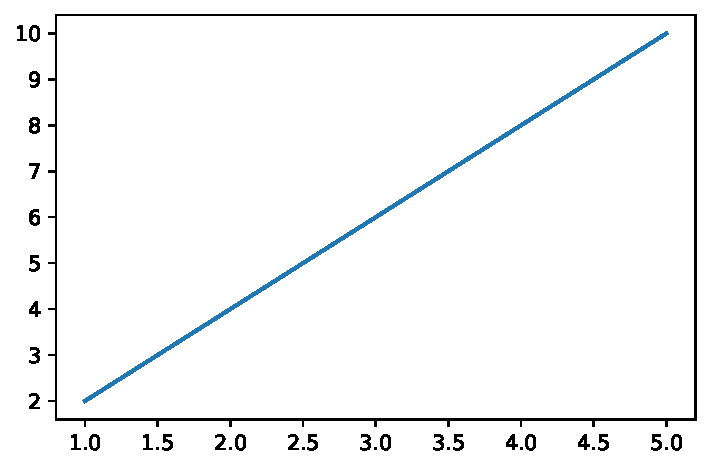
\includegraphics{index_files/figure-pdf/cell-2-output-1.pdf}

}

\end{figure}

\hypertarget{gruxe1ficos-de-barras}{%
\subsection{Gráficos de barras}\label{gruxe1ficos-de-barras}}

Los gráficos de barras son una excelente forma de representar datos
categóricos y comparar diferentes valores entre categorías. Son ideales
cuando queremos mostrar la relación entre una variable independiente
(categoría) y una variable dependiente (valor).

\textbf{Paso 1: Preparar los datos} Antes de crear el gráfico de barras,
necesitamos tener nuestros datos organizados. Asegúrate de tener una
lista o array con las categorías que deseas representar en el eje X, y
otra lista o array con los valores correspondientes en el eje Y.

\textbf{Paso 2: Crear el gráfico} Utilizaremos la función \texttt{bar()}
de Matplotlib para crear el gráfico de barras. Pasaremos nuestros datos
de los ejes X e Y como argumentos. A continuación, utilizaremos la
función \texttt{show()} para visualizar el gráfico.

\begin{Shaded}
\begin{Highlighting}[]
\ImportTok{import}\NormalTok{ matplotlib.pyplot }\ImportTok{as}\NormalTok{ plt}

\CommentTok{\# Datos de ejemplo}
\NormalTok{categorias }\OperatorTok{=}\NormalTok{ [}\StringTok{\textquotesingle{}A\textquotesingle{}}\NormalTok{, }\StringTok{\textquotesingle{}B\textquotesingle{}}\NormalTok{, }\StringTok{\textquotesingle{}C\textquotesingle{}}\NormalTok{, }\StringTok{\textquotesingle{}D\textquotesingle{}}\NormalTok{]}
\NormalTok{valores }\OperatorTok{=}\NormalTok{ [}\DecValTok{10}\NormalTok{, }\DecValTok{15}\NormalTok{, }\DecValTok{7}\NormalTok{, }\DecValTok{12}\NormalTok{]}

\CommentTok{\# Crear el gráfico de barras}
\NormalTok{plt.bar(categorias, valores)}

\CommentTok{\# Mostrar el gráfico}
\NormalTok{plt.show()}
\end{Highlighting}
\end{Shaded}

\begin{figure}[H]

{\centering 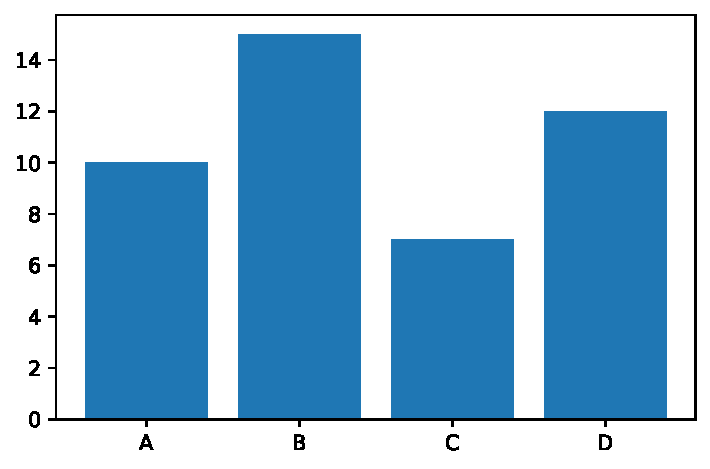
\includegraphics{index_files/figure-pdf/cell-3-output-1.pdf}

}

\end{figure}

\hypertarget{gruxe1ficos-de-dispersiuxf3n}{%
\subsection{Gráficos de dispersión}\label{gruxe1ficos-de-dispersiuxf3n}}

Los gráficos de dispersión son una excelente opción cuando queremos
visualizar la relación entre dos variables numéricas. Son especialmente
útiles para identificar patrones, tendencias o la existencia de alguna
correlación entre los datos.

\textbf{Paso 1: Preparar los datos} Antes de crear el gráfico de
dispersión, debemos asegurarnos de tener dos conjuntos de datos: uno
para el eje X (variable independiente) y otro para el eje Y (variable
dependiente). Asegúrate de que ambos conjuntos tengan la misma longitud
y correspondencia adecuada.

\textbf{Paso 2: Crear el gráfico} Utilizaremos la función
\texttt{scatter()} de Matplotlib para crear el gráfico de dispersión.
Pasaremos nuestros datos de los ejes X e Y como argumentos. Luego,
utilizaremos la función \texttt{show()} para visualizar el gráfico.

\begin{Shaded}
\begin{Highlighting}[]
\ImportTok{import}\NormalTok{ matplotlib.pyplot }\ImportTok{as}\NormalTok{ plt}

\CommentTok{\# Datos de ejemplo}
\NormalTok{x }\OperatorTok{=}\NormalTok{ [}\DecValTok{1}\NormalTok{, }\DecValTok{2}\NormalTok{, }\DecValTok{3}\NormalTok{, }\DecValTok{4}\NormalTok{, }\DecValTok{5}\NormalTok{]}
\NormalTok{y }\OperatorTok{=}\NormalTok{ [}\DecValTok{4}\NormalTok{, }\DecValTok{7}\NormalTok{, }\DecValTok{2}\NormalTok{, }\DecValTok{9}\NormalTok{, }\DecValTok{5}\NormalTok{]}

\CommentTok{\# Crear el gráfico de dispersión}
\NormalTok{plt.scatter(x, y)}

\CommentTok{\# Mostrar el gráfico}
\NormalTok{plt.show()}
\end{Highlighting}
\end{Shaded}

\begin{figure}[H]

{\centering 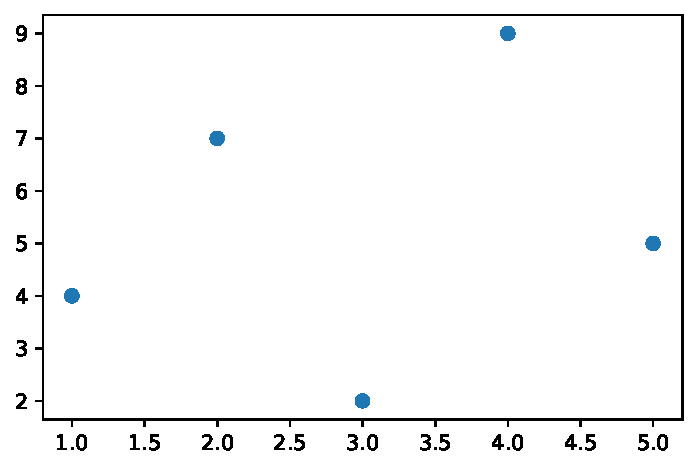
\includegraphics{index_files/figure-pdf/cell-4-output-1.pdf}

}

\end{figure}

\hypertarget{gruxe1ficos-de-uxe1rea}{%
\subsection{Gráficos de área}\label{gruxe1ficos-de-uxe1rea}}

Los gráficos de área son una forma efectiva de visualizar la
distribución o acumulación de datos a lo largo de una variable. Estos
gráficos son útiles cuando queremos mostrar la contribución relativa de
diferentes categorías o variables a un total.

\textbf{Paso 1: Preparar los datos} Antes de crear el gráfico de área,
debemos tener un conjunto de datos que represente las diferentes
categorías o variables que queremos visualizar. También necesitaremos
los valores correspondientes para cada categoría o variable.

\textbf{Paso 2: Crear el gráfico} Utilizaremos la función
\texttt{fill\_between()} de Matplotlib para crear el gráfico de área.
Pasaremos los datos de los ejes X e Y como argumentos y especificaremos
el color del área. Luego, utilizaremos la función \texttt{show()} para
visualizar el gráfico.

\begin{Shaded}
\begin{Highlighting}[]
\ImportTok{import}\NormalTok{ matplotlib.pyplot }\ImportTok{as}\NormalTok{ plt}

\CommentTok{\# Datos de ejemplo}
\NormalTok{x }\OperatorTok{=}\NormalTok{ [}\DecValTok{1}\NormalTok{, }\DecValTok{2}\NormalTok{, }\DecValTok{3}\NormalTok{, }\DecValTok{4}\NormalTok{, }\DecValTok{5}\NormalTok{]}
\NormalTok{y }\OperatorTok{=}\NormalTok{ [}\DecValTok{2}\NormalTok{, }\DecValTok{4}\NormalTok{, }\DecValTok{6}\NormalTok{, }\DecValTok{4}\NormalTok{, }\DecValTok{8}\NormalTok{]}

\CommentTok{\# Crear el gráfico de área}
\NormalTok{plt.fill\_between(x, y, color}\OperatorTok{=}\StringTok{\textquotesingle{}skyblue\textquotesingle{}}\NormalTok{)}

\CommentTok{\# Mostrar el gráfico}
\NormalTok{plt.show()}
\end{Highlighting}
\end{Shaded}

\begin{figure}[H]

{\centering 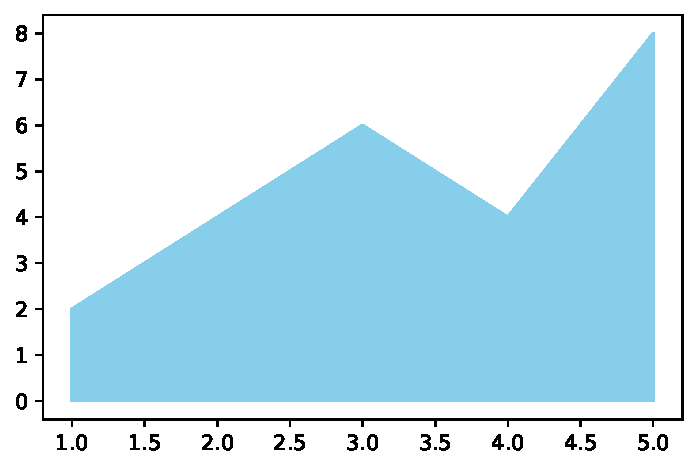
\includegraphics{index_files/figure-pdf/cell-5-output-1.pdf}

}

\end{figure}

\hypertarget{gruxe1ficos-de-pastel}{%
\subsection{Gráficos de pastel}\label{gruxe1ficos-de-pastel}}

Los gráficos de pastel son una forma popular de visualizar la proporción
de diferentes categorías o variables en un conjunto de datos. Estos
gráficos circulares son útiles para representar datos que se dividen en
partes proporcionales.

\textbf{Paso 1: Preparar los datos} Antes de crear el gráfico de pastel,
debemos tener un conjunto de datos con las categorías o variables que
queremos representar y los valores correspondientes para cada una de
ellas.

\textbf{Paso 2: Crear el gráfico} Utilizaremos la función \texttt{pie()}
de Matplotlib para crear el gráfico de pastel. Pasaremos los valores de
las categorías como argumentos y especificaremos los colores y etiquetas
correspondientes. Luego, utilizaremos la función \texttt{show()} para
visualizar el gráfico.

\begin{Shaded}
\begin{Highlighting}[]
\ImportTok{import}\NormalTok{ matplotlib.pyplot }\ImportTok{as}\NormalTok{ plt}

\CommentTok{\# Datos de ejemplo}
\NormalTok{categorias }\OperatorTok{=}\NormalTok{ [}\StringTok{\textquotesingle{}Manzanas\textquotesingle{}}\NormalTok{, }\StringTok{\textquotesingle{}Naranjas\textquotesingle{}}\NormalTok{, }\StringTok{\textquotesingle{}Plátanos\textquotesingle{}}\NormalTok{]}
\NormalTok{valores }\OperatorTok{=}\NormalTok{ [}\DecValTok{30}\NormalTok{, }\DecValTok{40}\NormalTok{, }\DecValTok{20}\NormalTok{]}

\CommentTok{\# Crear el gráfico de pastel}
\NormalTok{plt.pie(valores, labels}\OperatorTok{=}\NormalTok{categorias, colors}\OperatorTok{=}\NormalTok{[}\StringTok{\textquotesingle{}red\textquotesingle{}}\NormalTok{, }\StringTok{\textquotesingle{}orange\textquotesingle{}}\NormalTok{, }\StringTok{\textquotesingle{}yellow\textquotesingle{}}\NormalTok{])}

\CommentTok{\# Mostrar el gráfico}
\NormalTok{plt.show()}
\end{Highlighting}
\end{Shaded}

\begin{figure}[H]

{\centering 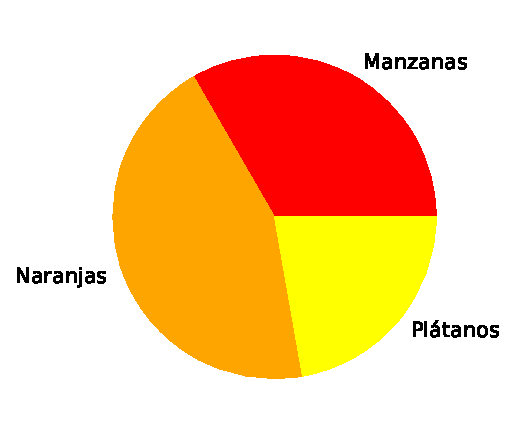
\includegraphics{index_files/figure-pdf/cell-6-output-1.pdf}

}

\end{figure}

\hypertarget{personalizaciuxf3n-de-gruxe1ficos}{%
\section{Personalización de
gráficos}\label{personalizaciuxf3n-de-gruxe1ficos}}

\hypertarget{cambio-de-colores-y-estilos}{%
\subsection{Cambio de colores y
estilos}\label{cambio-de-colores-y-estilos}}

La personalización de colores y estilos en los gráficos es una forma de
agregar tu toque personal y hacer que tus visualizaciones sean más
atractivas y significativas. Con Python, puedes cambiar fácilmente los
colores de las líneas, los puntos y las áreas en tus gráficos, así como
también aplicar diferentes estilos para resaltar la información más
relevante.

\textbf{Cambio de colores:}

Puedes cambiar los colores predeterminados de tus gráficos utilizando la
opción \texttt{color} en las funciones de trazado. Por ejemplo, si
deseas cambiar el color de una línea en un gráfico de línea, puedes
especificar un color diferente utilizando el argumento \texttt{color}
seguido del nombre del color o su código hexadecimal.

\begin{Shaded}
\begin{Highlighting}[]
\ImportTok{import}\NormalTok{ matplotlib.pyplot }\ImportTok{as}\NormalTok{ plt}

\CommentTok{\# Datos de ejemplo}
\NormalTok{x }\OperatorTok{=}\NormalTok{ [}\DecValTok{1}\NormalTok{, }\DecValTok{2}\NormalTok{, }\DecValTok{3}\NormalTok{, }\DecValTok{4}\NormalTok{]}
\NormalTok{y }\OperatorTok{=}\NormalTok{ [}\DecValTok{10}\NormalTok{, }\DecValTok{20}\NormalTok{, }\DecValTok{15}\NormalTok{, }\DecValTok{25}\NormalTok{]}

\CommentTok{\# Cambiar el color de la línea a rojo}
\NormalTok{plt.plot(x, y, color}\OperatorTok{=}\StringTok{\textquotesingle{}red\textquotesingle{}}\NormalTok{)}

\CommentTok{\# Mostrar el gráfico}
\NormalTok{plt.show()}
\end{Highlighting}
\end{Shaded}

\begin{figure}[H]

{\centering 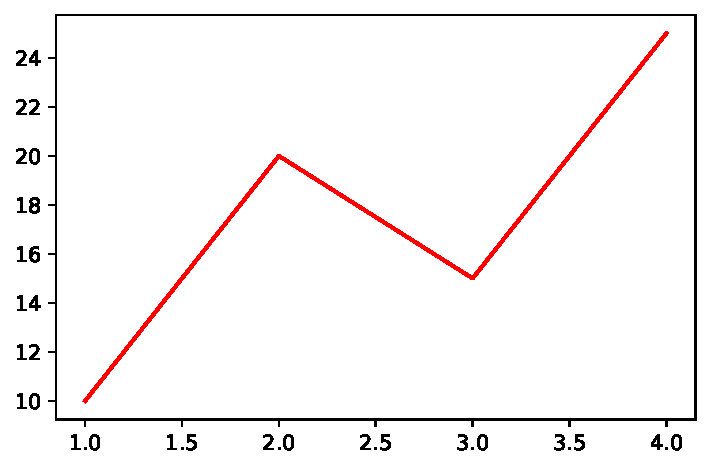
\includegraphics{index_files/figure-pdf/cell-7-output-1.pdf}

}

\end{figure}

Además de los colores predefinidos, también puedes utilizar códigos
hexadecimales para seleccionar colores personalizados. Por ejemplo,
\texttt{color=\textquotesingle{}\#FF0000\textquotesingle{}} representa
el color rojo.

\textbf{Cambio de estilos:}

Python también te permite cambiar el estilo de tus gráficos para
adaptarlos a tus preferencias. Puedes utilizar diferentes estilos
predefinidos, como \texttt{\textquotesingle{}seaborn\textquotesingle{}},
\texttt{\textquotesingle{}ggplot\textquotesingle{}},
\texttt{\textquotesingle{}fivethirtyeight\textquotesingle{}}, entre
otros. Simplemente utiliza la función \texttt{plt.style.use()} y pasa el
nombre del estilo que deseas aplicar.

\begin{Shaded}
\begin{Highlighting}[]
\ImportTok{import}\NormalTok{ matplotlib.pyplot }\ImportTok{as}\NormalTok{ plt}

\CommentTok{\# Estilo de gráfico \textquotesingle{}seaborn\textquotesingle{}}
\NormalTok{plt.style.use(}\StringTok{\textquotesingle{}seaborn\textquotesingle{}}\NormalTok{)}

\CommentTok{\# Datos y trazado del gráfico}
\NormalTok{x }\OperatorTok{=}\NormalTok{ [}\DecValTok{1}\NormalTok{, }\DecValTok{2}\NormalTok{, }\DecValTok{3}\NormalTok{, }\DecValTok{4}\NormalTok{]}
\NormalTok{y }\OperatorTok{=}\NormalTok{ [}\DecValTok{10}\NormalTok{, }\DecValTok{20}\NormalTok{, }\DecValTok{15}\NormalTok{, }\DecValTok{25}\NormalTok{]}
\NormalTok{plt.plot(x, y)}

\CommentTok{\# Mostrar el gráfico}
\NormalTok{plt.show()}
\end{Highlighting}
\end{Shaded}

\begin{figure}[H]

{\centering 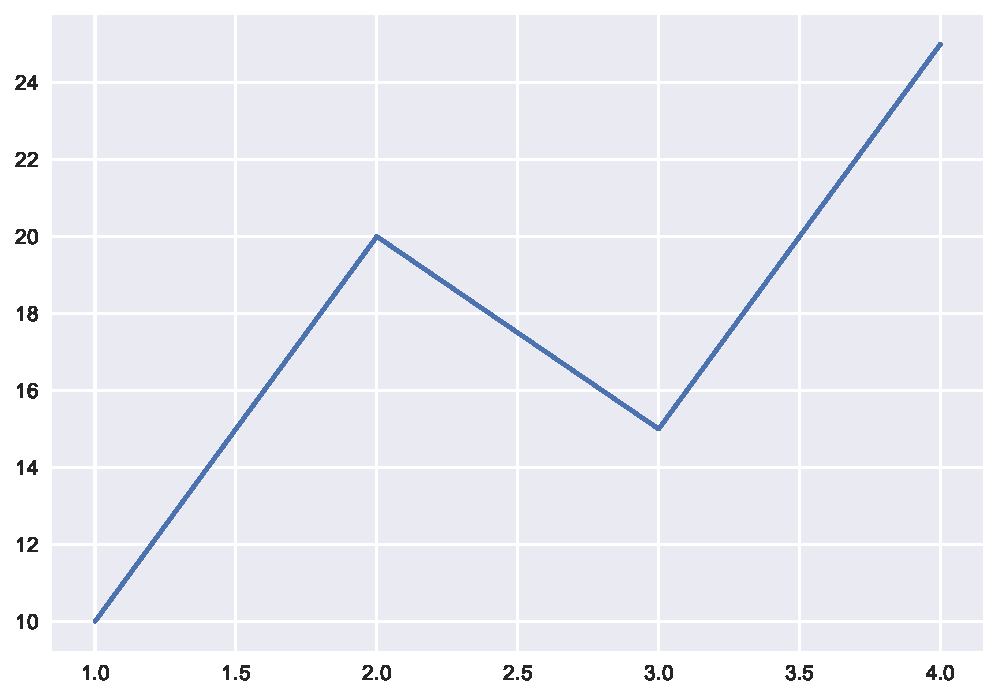
\includegraphics{index_files/figure-pdf/cell-8-output-1.pdf}

}

\end{figure}

Puedes experimentar con diferentes estilos y encontrar el que se ajuste
mejor a tus necesidades y preferencias.

\hypertarget{agregando-etiquetas-y-tuxedtulos}{%
\subsection{Agregando etiquetas y
títulos}\label{agregando-etiquetas-y-tuxedtulos}}

Las etiquetas y los títulos son elementos clave en tus gráficos, ya que
proporcionan información adicional y ayudan a interpretar los datos de
manera más clara. Python te ofrece varias opciones para agregar
etiquetas a los ejes, así como títulos para el gráfico en general.

\textbf{Etiquetas de ejes:}

Las etiquetas de ejes son fundamentales para comprender qué representan
los valores en los gráficos. Puedes agregar etiquetas a los ejes x e y
utilizando las funciones \texttt{plt.xlabel()} y \texttt{plt.ylabel()},
respectivamente. Simplemente pasa una cadena de texto como argumento
para describir cada eje.

\begin{Shaded}
\begin{Highlighting}[]
\ImportTok{import}\NormalTok{ matplotlib.pyplot }\ImportTok{as}\NormalTok{ plt}

\CommentTok{\# Datos de ejemplo}
\NormalTok{x }\OperatorTok{=}\NormalTok{ [}\DecValTok{1}\NormalTok{, }\DecValTok{2}\NormalTok{, }\DecValTok{3}\NormalTok{, }\DecValTok{4}\NormalTok{]}
\NormalTok{y }\OperatorTok{=}\NormalTok{ [}\DecValTok{10}\NormalTok{, }\DecValTok{20}\NormalTok{, }\DecValTok{15}\NormalTok{, }\DecValTok{25}\NormalTok{]}

\CommentTok{\# Trazado del gráfico}
\NormalTok{plt.plot(x, y)}

\CommentTok{\# Etiquetas de ejes}
\NormalTok{plt.xlabel(}\StringTok{\textquotesingle{}Eje X\textquotesingle{}}\NormalTok{)}
\NormalTok{plt.ylabel(}\StringTok{\textquotesingle{}Eje Y\textquotesingle{}}\NormalTok{)}

\CommentTok{\# Mostrar el gráfico}
\NormalTok{plt.show()}
\end{Highlighting}
\end{Shaded}

\begin{figure}[H]

{\centering 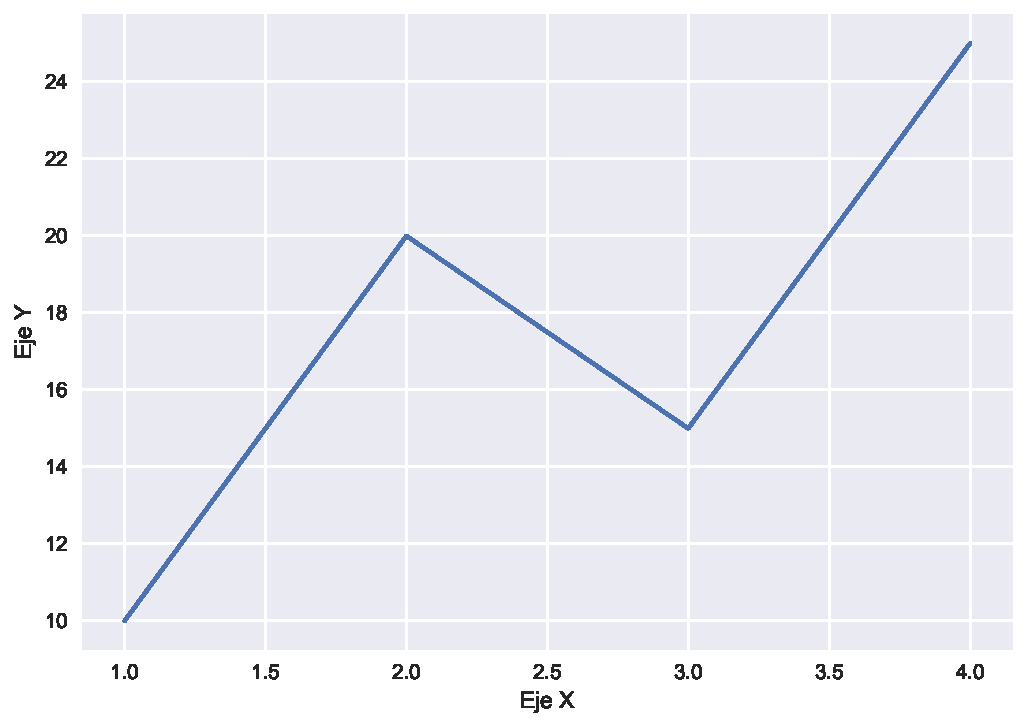
\includegraphics{index_files/figure-pdf/cell-9-output-1.pdf}

}

\end{figure}

Asegúrate de elegir etiquetas descriptivas que reflejen el contenido y
la interpretación de los datos en tus gráficos.

\textbf{Título del gráfico:}

El título del gráfico es útil para resumir la información principal o el
propósito del gráfico. Puedes agregar un título utilizando la función
\texttt{plt.title()} y pasando una cadena de texto como argumento.

\begin{Shaded}
\begin{Highlighting}[]
\ImportTok{import}\NormalTok{ matplotlib.pyplot }\ImportTok{as}\NormalTok{ plt}

\CommentTok{\# Datos de ejemplo}
\NormalTok{x }\OperatorTok{=}\NormalTok{ [}\DecValTok{1}\NormalTok{, }\DecValTok{2}\NormalTok{, }\DecValTok{3}\NormalTok{, }\DecValTok{4}\NormalTok{]}
\NormalTok{y }\OperatorTok{=}\NormalTok{ [}\DecValTok{10}\NormalTok{, }\DecValTok{20}\NormalTok{, }\DecValTok{15}\NormalTok{, }\DecValTok{25}\NormalTok{]}

\CommentTok{\# Trazado del gráfico}
\NormalTok{plt.plot(x, y)}

\CommentTok{\# Título del gráfico}
\NormalTok{plt.title(}\StringTok{\textquotesingle{}Gráfico de ejemplo\textquotesingle{}}\NormalTok{)}

\CommentTok{\# Mostrar el gráfico}
\NormalTok{plt.show()}
\end{Highlighting}
\end{Shaded}

\begin{figure}[H]

{\centering 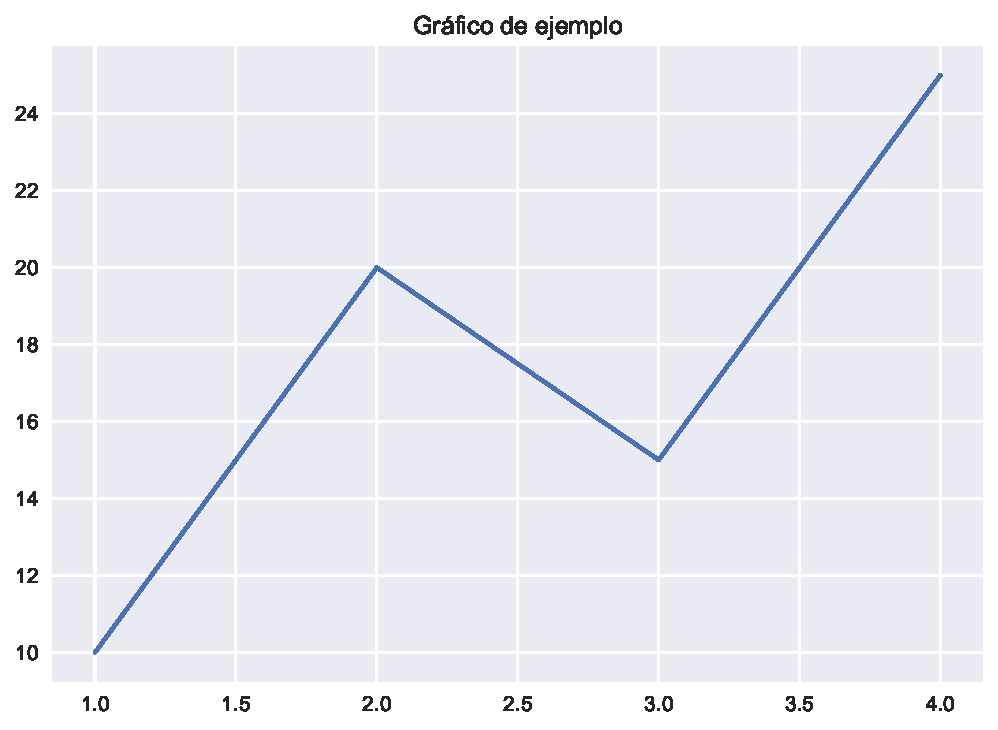
\includegraphics{index_files/figure-pdf/cell-10-output-1.pdf}

}

\end{figure}

Al igual que con las etiquetas de ejes, elige un título claro y conciso
que resuma la información que se muestra en el gráfico.

\hypertarget{configuraciuxf3n-de-ejes-y-leyendas}{%
\subsection{Configuración de ejes y
leyendas}\label{configuraciuxf3n-de-ejes-y-leyendas}}

La configuración de los ejes y las leyendas en tus gráficos es
fundamental para proporcionar más información y claridad a tus
visualizaciones. Python te ofrece diversas opciones para personalizar
los ejes y agregar leyendas que ayuden a interpretar tus gráficos de
manera efectiva.

\textbf{Personalización de ejes:}

Puedes personalizar los ejes de tu gráfico mediante la función
\texttt{plt.axis()}, que te permite establecer los límites de los ejes x
e y. Pasa una lista en el siguiente orden:
\texttt{{[}xmin,\ xmax,\ ymin,\ ymax{]}} para definir los límites de
cada eje.

\begin{Shaded}
\begin{Highlighting}[]
\ImportTok{import}\NormalTok{ matplotlib.pyplot }\ImportTok{as}\NormalTok{ plt}

\CommentTok{\# Datos de ejemplo}
\NormalTok{x }\OperatorTok{=}\NormalTok{ [}\DecValTok{1}\NormalTok{, }\DecValTok{2}\NormalTok{, }\DecValTok{3}\NormalTok{, }\DecValTok{4}\NormalTok{]}
\NormalTok{y }\OperatorTok{=}\NormalTok{ [}\DecValTok{10}\NormalTok{, }\DecValTok{20}\NormalTok{, }\DecValTok{15}\NormalTok{, }\DecValTok{25}\NormalTok{]}

\CommentTok{\# Trazado del gráfico}
\NormalTok{plt.plot(x, y)}

\CommentTok{\# Personalización de ejes}
\NormalTok{plt.axis([}\DecValTok{0}\NormalTok{, }\DecValTok{5}\NormalTok{, }\DecValTok{0}\NormalTok{, }\DecValTok{30}\NormalTok{])}

\CommentTok{\# Mostrar el gráfico}
\NormalTok{plt.show()}
\end{Highlighting}
\end{Shaded}

\begin{figure}[H]

{\centering 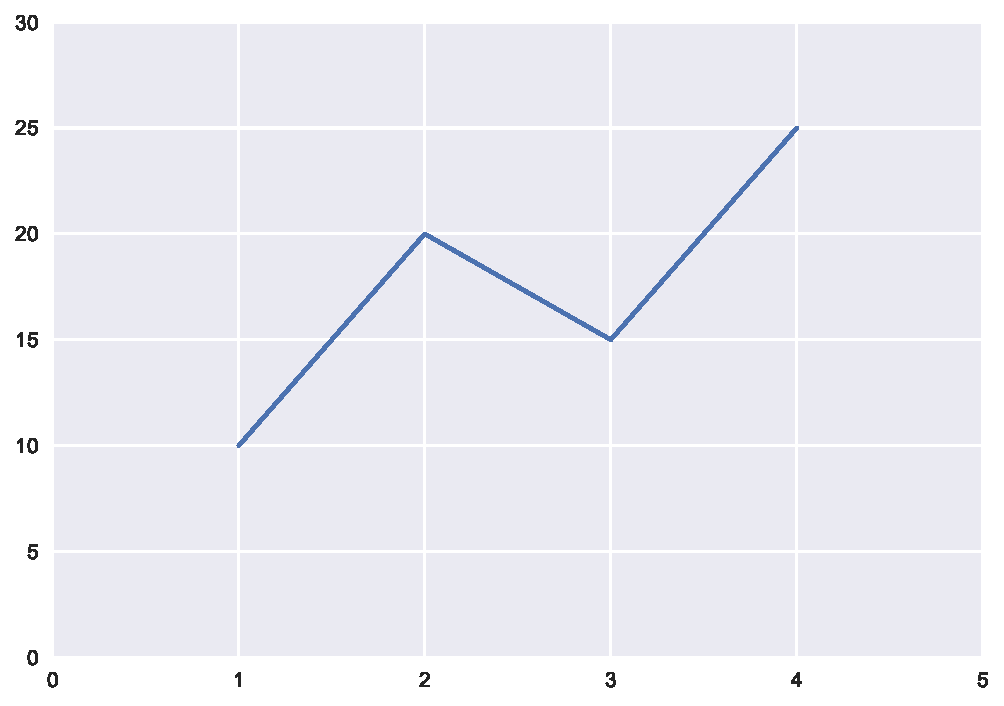
\includegraphics{index_files/figure-pdf/cell-11-output-1.pdf}

}

\end{figure}

Establecer límites adecuados en los ejes es importante para asegurarte
de que tus datos se muestren correctamente y se ajusten al espacio
disponible en el gráfico.

\textbf{Agregando leyendas:}

Las leyendas son útiles para identificar diferentes elementos en tus
gráficos, como líneas, barras o puntos. Puedes agregar una leyenda
utilizando la función \texttt{plt.legend()} después de trazar los
elementos en tu gráfico. Además, puedes especificar la ubicación de la
leyenda pasando un argumento como
\texttt{\textquotesingle{}upper\ right\textquotesingle{}},
\texttt{\textquotesingle{}lower\ left\textquotesingle{}}, etc.

\begin{Shaded}
\begin{Highlighting}[]
\ImportTok{import}\NormalTok{ matplotlib.pyplot }\ImportTok{as}\NormalTok{ plt}

\CommentTok{\# Datos de ejemplo}
\NormalTok{x }\OperatorTok{=}\NormalTok{ [}\DecValTok{1}\NormalTok{, }\DecValTok{2}\NormalTok{, }\DecValTok{3}\NormalTok{, }\DecValTok{4}\NormalTok{]}
\NormalTok{y1 }\OperatorTok{=}\NormalTok{ [}\DecValTok{10}\NormalTok{, }\DecValTok{20}\NormalTok{, }\DecValTok{15}\NormalTok{, }\DecValTok{25}\NormalTok{]}
\NormalTok{y2 }\OperatorTok{=}\NormalTok{ [}\DecValTok{5}\NormalTok{, }\DecValTok{15}\NormalTok{, }\DecValTok{10}\NormalTok{, }\DecValTok{20}\NormalTok{]}

\CommentTok{\# Trazado del gráfico}
\NormalTok{plt.plot(x, y1, label}\OperatorTok{=}\StringTok{\textquotesingle{}Serie 1\textquotesingle{}}\NormalTok{)}
\NormalTok{plt.plot(x, y2, label}\OperatorTok{=}\StringTok{\textquotesingle{}Serie 2\textquotesingle{}}\NormalTok{)}

\CommentTok{\# Agregar leyenda}
\NormalTok{plt.legend(loc}\OperatorTok{=}\StringTok{\textquotesingle{}upper right\textquotesingle{}}\NormalTok{)}

\CommentTok{\# Mostrar el gráfico}
\NormalTok{plt.show()}
\end{Highlighting}
\end{Shaded}

\begin{figure}[H]

{\centering 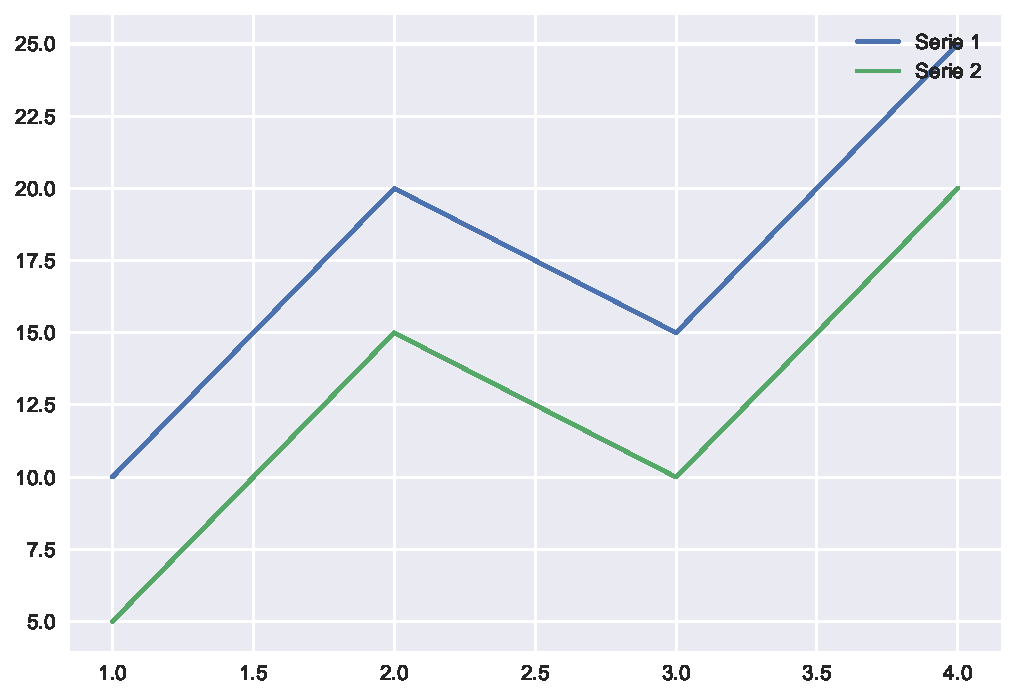
\includegraphics{index_files/figure-pdf/cell-12-output-1.pdf}

}

\end{figure}

Asegúrate de proporcionar etiquetas claras para cada serie de datos en
tu gráfico. Esto ayudará a los lectores a comprender qué representa cada
línea o elemento visualizado.

\hypertarget{auxf1adiendo-anotaciones-y-texto}{%
\subsection{Añadiendo anotaciones y
texto}\label{auxf1adiendo-anotaciones-y-texto}}

Las anotaciones y el texto son una forma poderosa de resaltar puntos
clave o proporcionar información adicional en tus gráficos. Python te
ofrece diversas opciones para añadir anotaciones y texto de manera
sencilla y efectiva.

\textbf{Anotaciones:}

Puedes añadir anotaciones en puntos específicos de tu gráfico utilizando
la función \texttt{plt.annotate()}. Esta función te permite colocar
texto en coordenadas específicas del gráfico. Puedes especificar las
coordenadas \texttt{xy} del punto donde deseas colocar la anotación y
las coordenadas \texttt{xytext} donde deseas que aparezca el texto.

\begin{Shaded}
\begin{Highlighting}[]
\ImportTok{import}\NormalTok{ matplotlib.pyplot }\ImportTok{as}\NormalTok{ plt}

\CommentTok{\# Datos de ejemplo}
\NormalTok{x }\OperatorTok{=}\NormalTok{ [}\DecValTok{1}\NormalTok{, }\DecValTok{2}\NormalTok{, }\DecValTok{3}\NormalTok{, }\DecValTok{4}\NormalTok{]}
\NormalTok{y }\OperatorTok{=}\NormalTok{ [}\DecValTok{10}\NormalTok{, }\DecValTok{20}\NormalTok{, }\DecValTok{15}\NormalTok{, }\DecValTok{25}\NormalTok{]}

\CommentTok{\# Trazado del gráfico}
\NormalTok{plt.plot(x, y)}

\CommentTok{\# Añadir una anotación}
\NormalTok{plt.annotate(}\StringTok{\textquotesingle{}Punto importante\textquotesingle{}}\NormalTok{, xy}\OperatorTok{=}\NormalTok{(}\DecValTok{2}\NormalTok{, }\DecValTok{20}\NormalTok{), xytext}\OperatorTok{=}\NormalTok{(}\DecValTok{3}\NormalTok{, }\DecValTok{22}\NormalTok{),}
\NormalTok{             arrowprops}\OperatorTok{=}\BuiltInTok{dict}\NormalTok{(arrowstyle}\OperatorTok{=}\StringTok{\textquotesingle{}{-}\textgreater{}\textquotesingle{}}\NormalTok{))}

\CommentTok{\# Mostrar el gráfico}
\NormalTok{plt.show()}
\end{Highlighting}
\end{Shaded}

\begin{figure}[H]

{\centering 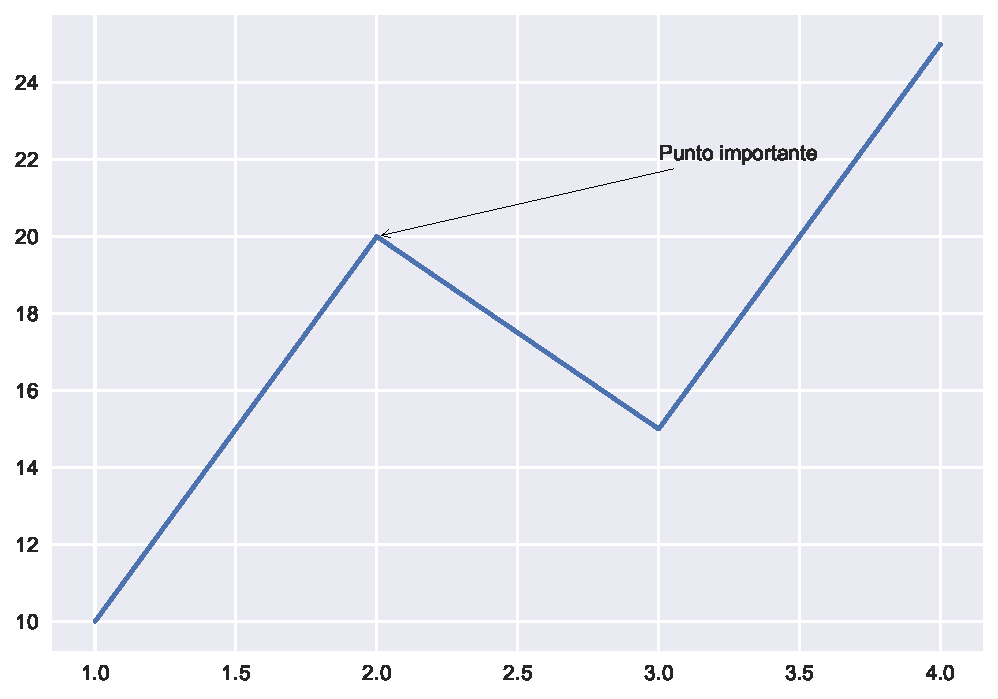
\includegraphics{index_files/figure-pdf/cell-13-output-1.pdf}

}

\end{figure}

Puedes personalizar aún más las anotaciones agregando flechas utilizando
el parámetro \texttt{arrowprops}. Esto puede ayudar a resaltar la
relación entre la anotación y el punto correspondiente en el gráfico.

\textbf{Texto:}

Además de las anotaciones, también puedes agregar texto en ubicaciones
específicas utilizando la función \texttt{plt.text()}. Esta función te
permite colocar texto en cualquier posición del gráfico especificando
las coordenadas \texttt{x} e \texttt{y} del punto donde deseas que
aparezca el texto.

\begin{Shaded}
\begin{Highlighting}[]
\ImportTok{import}\NormalTok{ matplotlib.pyplot }\ImportTok{as}\NormalTok{ plt}

\CommentTok{\# Datos de ejemplo}
\NormalTok{x }\OperatorTok{=}\NormalTok{ [}\DecValTok{1}\NormalTok{, }\DecValTok{2}\NormalTok{, }\DecValTok{3}\NormalTok{, }\DecValTok{4}\NormalTok{]}
\NormalTok{y }\OperatorTok{=}\NormalTok{ [}\DecValTok{10}\NormalTok{, }\DecValTok{20}\NormalTok{, }\DecValTok{15}\NormalTok{, }\DecValTok{25}\NormalTok{]}

\CommentTok{\# Trazado del gráfico}
\NormalTok{plt.plot(x, y)}

\CommentTok{\# Añadir texto}
\NormalTok{plt.text(}\DecValTok{2}\NormalTok{, }\DecValTok{20}\NormalTok{, }\StringTok{\textquotesingle{}Texto adicional\textquotesingle{}}\NormalTok{, fontsize}\OperatorTok{=}\DecValTok{12}\NormalTok{)}

\CommentTok{\# Mostrar el gráfico}
\NormalTok{plt.show()}
\end{Highlighting}
\end{Shaded}

\begin{figure}[H]

{\centering 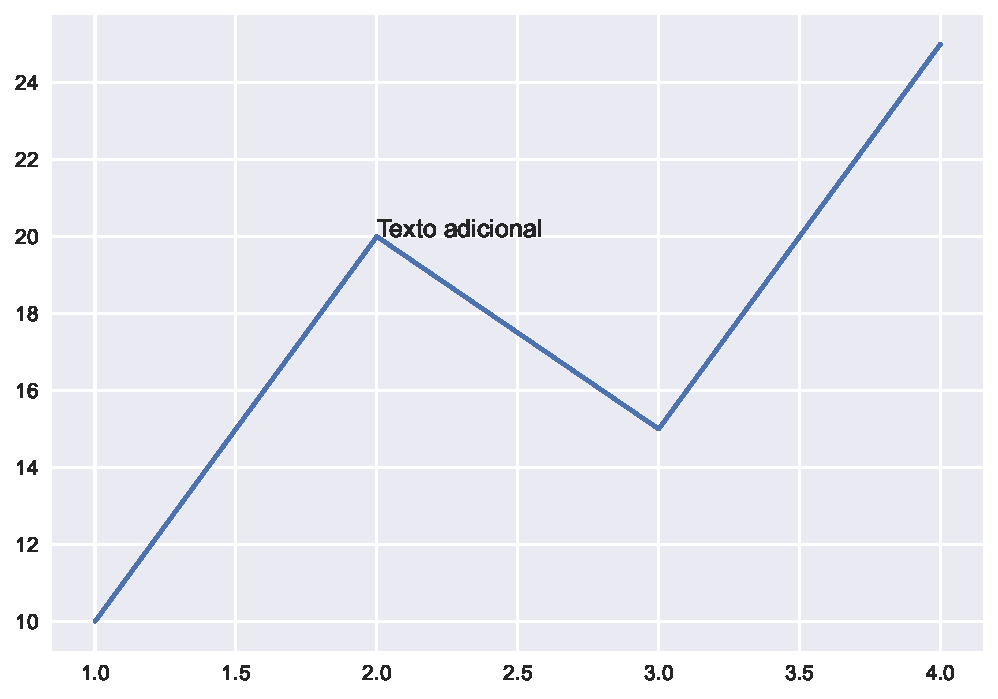
\includegraphics{index_files/figure-pdf/cell-14-output-1.pdf}

}

\end{figure}

Puedes ajustar el tamaño de la fuente del texto mediante el parámetro
\texttt{fontsize} para asegurarte de que sea legible y se ajuste a tu
gráfico.

\hypertarget{recursos-adicionales-y-pruxf3ximos-pasos}{%
\section{Recursos adicionales y próximos
pasos}\label{recursos-adicionales-y-pruxf3ximos-pasos}}

La visualización de datos con Python es un campo amplio y emocionante, y
hay muchos recursos disponibles para seguir aprendiendo y perfeccionando
tus habilidades. Aquí tienes algunos recursos adicionales que te pueden
ser útiles:

\hypertarget{enlaces-a-tutoriales-y-documentaciuxf3n}{%
\subsection{Enlaces a tutoriales y
documentación}\label{enlaces-a-tutoriales-y-documentaciuxf3n}}

\begin{itemize}
\item
  \textbf{Documentación oficial de Matplotlib}: La documentación oficial
  de Matplotlib es una fuente completa de información sobre la
  biblioteca. Puedes encontrar tutoriales, ejemplos de código y una guía
  detallada para aprovechar al máximo todas las funcionalidades que
  ofrece.
\item
  \textbf{Documentación oficial de Seaborn}: Si estás interesado en
  explorar más sobre Seaborn, la documentación oficial es un recurso
  invaluable. Aquí encontrarás ejemplos de gráficos, descripciones de
  las funciones y consejos para crear visualizaciones atractivas.
\item
  \textbf{Documentación oficial de Plotly}: Para aquellos que deseen
  adentrarse en la visualización de datos interactiva, Plotly ofrece una
  documentación detallada. Aprende cómo crear gráficos interactivos,
  agregar animaciones y personalizar tus visualizaciones.
\end{itemize}

\hypertarget{otras-fuentes-de-aprendizaje-y-comunidad}{%
\subsection{Otras fuentes de aprendizaje y
comunidad}\label{otras-fuentes-de-aprendizaje-y-comunidad}}

\begin{itemize}
\item
  \textbf{Cursos en línea}: Existen plataformas en línea que ofrecen
  cursos especializados en visualización de datos con Python. Algunos
  sitios populares incluyen Coursera, Udemy y DataCamp. Estos cursos te
  brindarán una base sólida y te guiarán a través de ejemplos prácticos.
\item
  \textbf{Foros y comunidades}: Únete a comunidades en línea dedicadas a
  la visualización de datos, como el subreddit r/dataisbeautiful o los
  grupos de LinkedIn especializados. Estos espacios te permitirán
  conectarte con otros entusiastas de la visualización de datos, hacer
  preguntas y obtener consejos valiosos.
\item
  \textbf{Libros y recursos impresos}: Explora libros dedicados a la
  visualización de datos en Python, como ``Python for Data Analysis'' de
  Wes McKinney o ``Python Data Science Handbook'' de Jake VanderPlas.
  Estos recursos ofrecen una visión más detallada y práctica de la
  visualización de datos.
\end{itemize}

¡Recuerda que la práctica constante es clave para mejorar tus
habilidades en la visualización de datos! No dudes en experimentar con
diferentes conjuntos de datos, probar nuevas técnicas y explorar las
posibilidades que Python ofrece en este campo.

En este blog, hemos cubierto una amplia gama de temas relacionados con
la visualización de datos en Python. Espero que hayas encontrado
información útil y te sientas inspirado para explorar y crear
visualizaciones impactantes. ¡No dudes en compartir tus creaciones y
experiencias con la comunidad!

Si tienes alguna pregunta o necesitas más recursos, ¡no dudes en
comunicarte! ¡Feliz visualización de datos!

\hypertarget{publicaciones-similares}{%
\section{Publicaciones Similares}\label{publicaciones-similares}}

Si te interesó este artículo, te recomendamos que explores otros blogs y
recursos relacionados que pueden ampliar tus conocimientos. Aquí te dejo
algunas sugerencias:

\begin{enumerate}
\def\labelenumi{\arabic{enumi}.}
\item
  \href{../2023-06-22-01-introduccion-a-python/index.qmd}{Introducción}
\item
  \href{../2023-06-23-02-variables-expresiones-y-statements-con-python/index.qmd}{Variables,
  expresiones y statements}
\item
  \href{../2023-06-24-03-objetos-de-python/index.qmd}{Objetos de Python}
\item
  \href{../2023-06-25-04-ejecucion-condicional-con-python/index.qmd}{Ejecución
  condicional}
\item
  \href{../2023-06-26-05-iteraciones-con-python/index.qmd}{Iteraciones}
\item
  \href{../2023-06-27-06-funciones-con-python/index.qmd}{Funciones}
\item
  \href{../2023-06-28-07-dataframes-con-python/index.qmd}{Dataframes}
\item
  \href{../2023-06-29-introduccion-a-la-visualizacion-de-datos-con-python/index.qmd}{Introducción
  a la visualización de datos}
\item
  \href{../2023-06-30-graficos-avanzados-con-python/index.qmd}{Gráficos
  avanzados}
\item
  \href{../2023-07-01-visualizacion-de-datos-en-tiempo-real-con-python/index.qmd}{Visualización
  de datos en tiempo real}
\item
  \href{../2023-07-02-visualizacion-de-datos-en-finanzas-con-python/index.qmd}{Visualización
  de datos en finanzas}
\item
  \href{../2023-07-03-visualizacion-de-datos-en-microeconomia-con-python/index.qmd}{Visualización
  de datos en microeconomía}
\item
  \href{../2023-07-04-visualizacion-de-datos-en-macroeconomia-con-python/index.qmd}{Visualización
  de datos en macroeconomía}
\item
  \href{../2023-07-05-visualizacion-de-datos-en-estadistica-con-python/index.qmd}{Visualización
  de datos en estadística}
\item
  \href{../2023-07-06-visualizacion-de-datos-en-econometria-con-python/index.qmd}{Visualización
  de datos en econometría}
\item
  \href{../2023-07-07-mejores-practicas-y-consejos-de-visualizacion-de-datos-con-python/index.qmd}{Mejores
  prácticas y consejos de visualización de datos}
\item
  \href{../2023-07-08-08-prediccion-y-metrica-de-performance-con-python/index.qmd}{Predicción
  y métrica de performance}
\item
  \href{../2023-07-09-09-metodos-de-machine-learning-para-clasificacion-con-python/index.qmd}{Métodos
  de machine learning para clasificación}
\item
  \href{../2023-07-10-10-metodos-de-machine-learning-para-regresion-con-python/index.qmd}{Métodos
  de machine learning para regresión}
\item
  \href{../2023-07-11-11-validacion-cruzada-y-composicion-del-modelo-con-python/index.qmd}{Validación
  cruzada y composición del modelo}
\end{enumerate}

Esperamos que encuentres estas publicaciones igualmente interesantes y
útiles. ¡Disfruta de la lectura!


\printbibliography


\end{document}
